\chapter{Desenvolvimento do projeto}\label{cap4}

Este capítulo descreve o projeto atribuído no estágio e o seu desenvolvimento, sendo este o capítulo mais longo, mas consequentemente o mais importante e o mais complexo.

\section{Introdução}

Como anteriormente referido foi destacada a tarefa de implementação de um projeto no estágio. Este projeto consiste no desenvolvimento de um software que permite a gestão das especificações de Webshops.

Estas Webshops são, como o nome indica, as lojas online as quais são clientes da Optiply. Estas lojas online são responsáveis por fornecer os produtos que os clientes compram e a Optiply é responsável por fornecer a gestão inteligente dos produtos em stock.

O trabalho foi recebido num \textit{.pdf}, numa reunião por video-conferencia, com o coordenador do estágio (Fábio Belga), um dos seus subordinados (André Figueira) que ficou encarregado de orientar os estagiários de Backend, e os mesmos (o autor deste relatório, Gonçalo Amaro e o estagiário da universade de Évora, José Azevedo), tendo esta reunião ocorrido após a fase formativa do \textit{Onboarding} descrita no capítulo anterior.

Assim, as primeiras secções deste capítulo servem como uma apresentação do projeto desenvolvido.

\section{Objetivos}

O objetivo deste projeto foi desenvolver um microserviço que permitisse a gestão das especificações de Webshops, contudo, o verdadeiro objetivo deste projeto é fornecer treino ao estagiário nas tecnologias da \textit{Tech Stack} da empresa, ou pelo menos num dos seus projetos.

\newpage

A \textit{Tech Stack} referida é a seguinte:

\begin{itemize}
  \item Micronaut: Framework de desenvolvimento de microserviços.
  \item Java: Linguagem de programação.
  \item Gradle: Sistema de gestão de dependências e tarefas.
  \item jOOQ: Framework de código-fonte para acesso a bases de dados.
  \item Flyway: Framework de migração de bases de dados.
  \item PostgreSQL: Sistema de bases de dados.
  \item Junit5 (Spock também é aceitável): Framework de testes.
  \item Mockito: Framework de auxiliar a testes via simulação.
\end{itemize}

Para desenvolver este microserviço temos de saber variados conjuntos de informação. Uns técnicos e outros específicos ao projeto, nomeadamente:

\noindent\ \bullet\ Ter conhecimento sobre a especificação de REST, que é um protocolo de comunicação entre aplicações via pedidos HTTP, com \textit{standards} de resposta em \textit{status} codes mas ainda assim flexíveis;

\noindent\ \bullet\ Que cada Webshop têm um conjunto de especificações, das quais representam informações e estados relevantes à entidade que esta refere. As quais são:

\begin{itemize}
  \item \textit{URL:} URL da loja online, têm validação e requer protocolo na URL;
  \item \textit{Handle:} identificador único da loja online;
  \item \textit{Interest Rate:} taxa de juros que a loja online paga, 20\% é o valor por defeito;
  \item \textit{Service Level Categories:} categorias de níveis de serviço que a loja têm, são três categorias (A,B e C) e as suas somas requerem ser iguais a 100\%;
  \item \textit{Contact Email List:} lista de emails de contacto da loja online, têm validação;
  \item \textbf{Extra:} \textit{Settings:} configurações da loja online:
    \begin{itemize}
      \item \textit{Enable Multi Supplier:} permite múltiplos fornecedores;
      \item \textit{Enable Run Jobs:} permite execução de tarefas;
      \item \textit{Currency:} moeda da loja online em ISO-4217;
    \end{itemize}
\end{itemize}

Sendo que as ultimas especificações (as \textit{Settings}) são Extras, ou seja, não são obrigatórias, mas foram implementadas.

\newpage

O microserviço tem um determinado conjunto de tarefas a cumprir as quais são:

\begin{itemize}
  \item Obter uma única Webshop;
  \item Pesquisa de Webshops:
    \begin{itemize}
      \item Deve ser capaz de ordenar e filtrar por qualquer campo da tabela;
      \item Só é necessário ordenar por um único campo. Os resultados devem ser consistentes com cada pedido. (Se ordenar por Taxa de Juros, como pode-se garantir que os mesmos resultados sejam obtidos em todos os pedidos?)
      \item Só é necessário filtrar por um único campo. Os filtros suportados são:
        \begin{itemize}
          \item ``:'' significa \textit{Igual}. Exemplo: handle:optiply
          \item ``\%'' significa \textit{ILIKE} (semelhante, \textit{case-insensitive}).\\Exemplo: handle\%optiply
          \item \textbf{Extra:} ``>'' significa \textit{Maior Que}. Exemplo: interestRate>20
          \item \textbf{Extra:} ``<'' significa \textit{Menor Que}. Exemplo: interestRate<20
        \end{itemize}
    \end{itemize}
  \item Apagar uma única Webshop.
  \item Criar uma única Webshop.
  \item Atualizar qualquer campo da Webshop.
  \item \textbf{Extra:} Filtrar por múltiplos campos.
  \item \textbf{Extra:} Criar múltiplas Webshops.
  \item \textbf{Extra:} Obter as configurações da Webshop.
  \item \textbf{Extra:} Atualizar as configurações da Webshop.
\end{itemize}

Tendo sempre em conta que os resultados devem ser idempotentes e no seu estado mais recente e que os pedidos HTTP devem retornar:

\begin{itemize}
  \item Criar deve retornar o \textit{status code} 201.
  \item Obter e Atualizar devem retornar o \textit{status code} 200.
  \item Apagar deve retornar o \textit{status code} 204.
  \item Qualquer pedido deve retornar o \textit{status code} 404 se a loja não existir.
  \item Qualquer outro erro interno deve retornar o \textit{status code} 500 (Erro Interno).
\end{itemize}

\newpage

\section{Implementação}

\subsection{Pré-Requisitos}

Para começar a implementar a API, precisa-se de um conjunto de ferramentas. Essas ferramentas passam por um JDK (um SDK de Java), otimamente algo aberto e conforme os standards de \href{https://openjdk.org/}{OpenJDK}, tendo sido utilizado o \href{https://docs.aws.amazon.com/corretto/latest/corretto-17-ug/downloads-list.html}{Amazon Corretto}\cite{corretto}, visto à sua licença ser aberta e gratuita, multiplataforma e vem com suporte de longo prazo que incluirá melhorias de desempenho e correções de segurança.

Para gestão de pacotes e tarefas, precisou-se de um gestor de pacotes, tendo sido utilizado o \href{https://gradle.org/}{Gradle}, e como um dos meus computadores de trabalho usa \href{https://www.microsoft.com/pt-pt/software-download/windows10} em vez de \href{https://archlinux.org/download/}{Linux}, a instalação do \href{https://gradle.org/}{Gradle} sem um gestor de pacotes e alteração do path, facilitou usar um IDE que trate desses assuntos, o qual foi recomendado o \href{https://www.jetbrains.com/idea/}{IntelliJ IDEA} da \href{https://www.jetbrains.com/}{JetBrains}.

Para hospedar a base de dados e o projeto, numa pequena rede de containers interna, foi instalado o \href{https://www.docker.com/}{Docker} no \textit{desktop} \href{https://www.microsoft.com/pt-pt/software-download/windows10}{Windows} (e utilizado o \href{https://podman.io/}{Podman} no portátil \href{https://archlinux.org/download/}{Linux}, pelo simples facto de já o ter instalado previamente).

No entanto ainda falta algo bastante importante. Nomeadamente, algo que faça o Bootstrap do projeto em \href{https://micronaut.io/}{Micronaut}, para isso temos variadas opções:

\begin{itemize}
  \item Ir ao o \href{https://micronaut.io/launch}{Micronaut Launch Website}
  \item Usar o \href{https://micronaut.io/download/}{Micronaut CLI} \href{https://micronaut-projects.github.io/micronaut-starter/latest/guide/index.html}{(em que temos aqui a documentação)}
  \item Fazer \href{https://curl.se/}{curl} à API do \href{https://launch.micronaut.io/create/default/com.optiply.project.webshop?lang=JAVA&build=GRADLE&test=JUNIT&javaVersion=JDK_17&features=jackson-databind&features=kubernetes-reactor-client&features=properties&features=flyway&features=jdbc-hikari&features=jooq&features=postgres&features=r2dbc&features=testcontainers&features=lombok&features=mockito&features=openrewrite&features=asciidoctor&features=logback&features=reactor&features=security-jwt&features=problem-json&features=jackson-xml}{Micronaut Launch}
\end{itemize}

O qual nenhum foi necessário pela razão estabelecidade na subsecção imediatamente seguinte.

\subsection{Inicio do Projeto}

Neste caso em especifico foi fornecido um repositório privado no \href{https://bitbucket.org/}{BitBucket}, o qual apenas foi necessário fazer uma \textit{fork}. O estado desse repositório e da \textit{fork} pode ser visto no neste \href{https://github.com/CatKinKitKat/MicronautJooqPostgresREST/tree/07d359ce933dde634f176dc95bf5ac1b3e4bc93d}{\textit{commit}} (\href{https://github.com/CatKinKitKat/MicronautJooqPostgresREST}{num repositório do autor} do \href{https://github.com/}{GitHub}, onde no projeto foi adicionado como segunda origem, para backup \cite{backup}).

Nesta diretoria de projeto nos atribuída, foi calculada que era maior e mais complicada que o necessário, talvez esta seja única e o que varia são os projetos que a usam. Com isso em conta foi decido, fazer uma redução ao projeto, para que ficasse mais simples de trabalhar e não houvessem pacotes ou funcionalidades que não fossem necessárias.

Após a redução, o projeto ficou com apenas dois subprojetos para o Gradle gerir, um que contem a aplicação em sí e o outro que trata dos repositórios/classes de transações à base de dados. O numero de pacotes externos e funcionalidades foi reduzido para o mínimo necessário, esses incluíram: \href{https://flywaydb.org/}{Flyway}, \href{http://fasterxml.com/}{Jackson}, \href{https://www.jooq.org/}{jOOQ}, \href{https://junit.org/junit5/}{JUnit}, \href{https://logback.qos.ch/}{Logback}, \href{https://projectlombok.org/}{Lombok}, \href{https://site.mockito.org/}{Mockito}, \href{https://jdbc.postgresql.org/}{Postgres}, \href{https://r2dbc.io/}{R2DBC} e \href{https://projectreactor.io/}{Reactor}.

\subsubsection{Detalhes sobre as tecnologias}

\paragraph{\href{https://flywaydb.org/}{Flyway}\\}

O \href{https://flywaydb.org/}{Flyway} é um framework de migrações de bases de dados, que é usado para gerênciar as migrações de bases de dados de projetos Java. Funciona de maneira semelhante às migrações nativas do ASP.NET Core.\cite{flyway}

Este pacote adiciona essas capacidades a tarefas do Gradle, como o \textit{flywayMigrate} e \textit{flywayInfo}. A migrações são feitas através de um ficheiro de migrações, que é um ficheiro de SQL, dentro da diretoria de migrações (\textit{PROJECT\_ROOT/src/main/resources/db/migrations}), com a versão em que a migração deve ser executada e dois \textit{underscores}.

\paragraph{\href{http://fasterxml.com/}{Jackson}\\}

O \href{http://fasterxml.com/}{Jackson} é um framework de serialização de objetos, que é usado para serializar objetos em JSON.\cite{jackson}

A serialização é um processo de transformação de um objeto em um JSON, e a deserialização é o processo de transformação de um JSON em um objeto.

Isto é feito principalmente através de um objeto \textit{ObjectMapper}, que é um objeto que implementa a interface \textit{com.fasterxml.jackson.databind.ObjectMapper}.

\paragraph{\href{https://jooq.org/}{jOOQ}\\}

O \href{https://jooq.org/}{jOOQ} é um framework de código-fonte de código-aberto, que é usado para gerir a base de dados. Este funciona de maneira semelhante às operações do Entity Framework Core para ASP.NET Core, sendo que este abstrai as operações de SQL em wrappers programáticos.\cite{jooq}

\paragraph{\href{https://junit.org/junit5/}{JUnit}\\}

O \href{https://junit.org/junit5/}{JUnit} é um framework de testes, que é usado para gerênciar os testes de unidades. Usado muito na disciplina de Programação Orientada a Objetos.\cite{junit}

\paragraph{\href{https://logback.qos.ch/}{Logback}\\}

O \href{https://logback.qos.ch/}{Logback} é um framework de logging, que é usado para gerir os logs de um projeto, com o foco em abstrair o uso de logs ao mais simples possível. É o sucessor do \href{https://log4j.org/}{Log4j}, que foi alvo de uma vulnerabilidade recentemente.\cite{logback}

No Windows devemos alterar uma configuração: a desativação do JANSI, que não funciona com alguns Locales, em especial os que o Windows usa.

\paragraph{\href{https://projectlombok.org/}{Lombok}\\}

O \href{https://projectlombok.org/}{Lombok} é um framework de código-fonte de código-aberto, que é usado para gerir a criação de classes de objetos através de anotações. Com estas anotações, abstraímos o código, evitamos repetição e automatizamos muito o processo desenvolvimento.\cite{lombok}

Por exemplo a anotação \textit{@Getter} faz com que o Java crie automaticamente os getters. Ou, a anotação \textit{@Data} faz com que o Java crie automaticamente os getters, setters, equals, hashCode, toString e clone.

\paragraph{\href{https://site.mockito.org/}{Mockito}\\}

O \href{https://site.mockito.org/}{Mockito} é um framework auxiliar de testes, que é usado para gerir os mocks de objetos. Os mocks são objetos que são usados para simular o comportamento de objetos realmente existentes.\cite{mockito}

Com os mocks, podemos testar objetos que ainda não existem, como um objeto de um repositório de dados, ou um objeto de um serviço. Como também isolamos o comportamento dos objetos, evitamos que os objetos sejam alterados durante o teste ou para testar apenas o comportamento do que comunica com o mesmo.

\paragraph{\href{https://jdbc.postgresql.org/}{PostgreSQL JDBC}\\}

O \href{https://jdbc.postgresql.org/}{PostgreSQL JDBC} é um driver JDBC, que é usado para conectar a bases de dados PostgreSQL. Um driver JDBC é um driver que permite ao Java a comunicação com bases de dados.\cite{postgresql}

PostgreSQL é o tipo de base de dados usado no projeto.

\paragraph{\href{https://r2dbc.io/}{R2DBC}\\}

O \href{https://r2dbc.io/}{R2DBC} é um driver de conexão à base de dados, mas contrariamente ao anterior este permite fazer transações reativas como as do Project Reactor ou do RxJava.\cite{r2dbc}

\paragraph{\href{https://projectreactor.io/}{Reactor}\\}

O \href{https://projectreactor.io/}{Reactor} é um framework de eventos, que é usado para gerir eventos e criar aplicações reativas. Uma aplicação reativa é uma aplicação que é executada num fluxo de eventos.\cite{reactor}

\subsection{Paradigma de Programação}

Programação reativa é o acto de programar para trabalhar com fluxos de dados assíncronos. Isto é importante devido o crescimento da Internet e a demanda enorme de dados em tempo real. Esta programação precisa de ser dinâmica, ou seja; diferente das formas tradicionais de desenvolvimento.\cite{reactive}

\newpage

Nas formas tradicionais de programar/desenvolver, de modo \textbf{muito} genérico, cria-se variadas tarefas e comunicam apenas em tempos pré-determinados, com respostas pré-determinadas, são ``rígidas'' e seguem regras diretas.

Isto funciona e continua a ser utilizado nos dias de hoje, no entanto, esta ``lógica'' não é compatível com as necessidades de alguns serviços atuais e os seus inúmeros clientes e dados. Na programação reativa isto ocorre de uma forma semelhante, mas mais inteligente, interligada em paralelo, sem seguir uma ordem cronológica e linear.

Os pilares da programação reativa são:

\begin{itemize}
  \item \textbf{Elástico:} Reage à demanda/carga: aplicações podem fazer uso de múltiplos núcleos e múltiplos servidores;
  \item \textbf{Resiliente:} Reage às falhas; aplicações reagem e se recuperam de
    falhas de software, hardware e de conectividade;
  \item \textbf{Message Driven:} Reage aos eventos (event driven): em vez de compor
    aplicações por múltiplas threads síncronas, sistemas são compostos de gerenciadores de eventos assíncronos e não bloqueantes;
  \item \textbf{Responsivo:} Reage aos utilizadores: aplicações que oferecem interações
    ricas e ``tempo real'' com utilizadores.
\end{itemize}

\subsection{Estrutura do Projeto}

A estrutura do projeto, como dito anteriormente, foi herdada da estrutura inicial vinda do repositório oferecido para \textit{forking}. Este projeto consistiu num projeto Gradle com três subprojetos: um pacote com classes estendidas de Monos, um pacote para o core do projeto, e um pacote para os repositórios que tratam das transações com a base de dados.

Sendo que as classes eram apenas \textit{MonoVoid}, \textit{MonoFalse} e \textit{MonoTrue} que simplesmente implementavam a interface \textit{Mono} e retornavam um valor booleano (ou nenhum), decidi cortá-las visto que não trazem quais quer nova funcionalidade ao projeto e não me custa escrever \textit{Mono<Boolean>} e retornar um valor booleano.

Com isto, a estrutura do projeto foi alterada para um projeto Gradle com dois subprojetos.

\subsection{Metodologia de desenvolvimento}

Foi notificado que o projeto seria desenvolvido de forma livre, sem qualquer metodologia de desenvolvimento. No entanto, sendo eu um alguém novo na area e a trabalhar remotamente, decidi que é extremamente importante arranjar um ambiente de desenvolvimento que me permita trabalhar, ponto. Por isto, decidi referir às estratégias de gestão de projeto ensinadas na disciplina de Engenharia de Software, como o \textit{Scrum} e o \textit{Kanban}.

Sabendo que esta empresa usa \textit{Scrum}, ponderou-se usar o mesmo e as ferramentas disponíveis no \href{https://www.atlassian.com/}{Atlassian} como \textit{Jira} e \textit{Confluence}; mas acabou por ser decidido usar uma estratégia menos rígida, o \textit{Kanban}.

\subsubsection{Kanban}

Para o projeto, a estratégia de desenvolvimento foi o \textit{Kanban}, ou pelo menos uma forma primitiva do mesmo. Expandindo, foi feito um quadro de tarefas divididas em cinco colunas: \textit{Tarefas}, \textit{Por aprender}, \textit{Por implementar} \textit{Por testar} e \textit{Terminadas}.

A metodologia de trabalho começava por ir identificando tarefas, se muito complexas dividi-las em pequenas tarefas e julgando a minha capacidade de as fazer. Colocando na coluna respetiva e depois trabalhando de acordo com o estado do quadro.

Este quadro infelizmente já não está acessível, pois a conta empresarial já foi fechada e não houve \textit{backup}. No entanto a \textbf{Figura 4.1} exemplifica o quadro de tarefas.

\begin{figure}[!hbt]
  \centering
  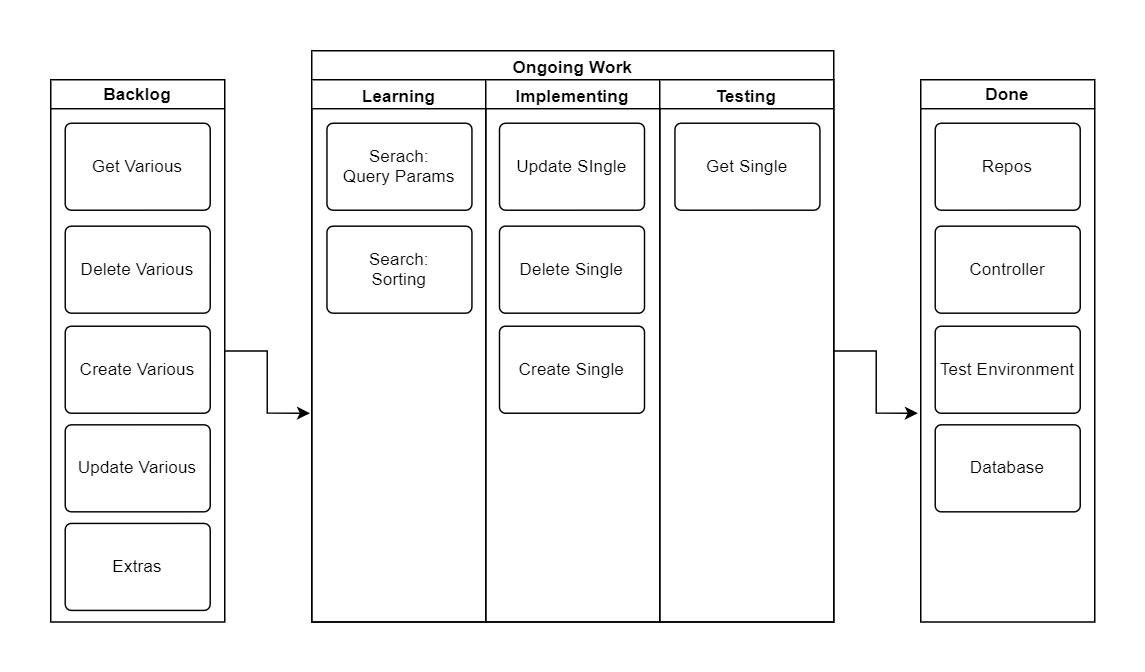
\includegraphics[width=14cm]{figuras/kanban.png}
  \caption{Exemplo do quadro Kanban, criado no \href{https://gitmind.com/app/flowchart/e7311869657}{GitMind}}
  \label{fig:kanban}
\end{figure}
\FloatBarrier

\subsubsection{Nota sobre a escolha}

Numa opinião subjetiva, a escolha do \textit{Kanban} sobre \textit{Scrum}, foi uma boa decisão, visto que o \textit{Scrum} é um padrão mais rígido e linear, havendo a (extra) necessidade em criar \textit{user-stories} e em definir \textit{sprints}. Já o \textit{Kanban} é um padrão mais flexível, tanto por ter menos etapas para organizar como por ter um quadro de tarefas menos \textit{standard} e mais flexível.

\subsection{Testes}

Para testar o software, foi recomendado uma mistura de \textit{JUnit} e \textit{Mockito} ou usar \textit{Spock}. Estes testes foram feitos dentro do subprojeto principal, e foram divididos em duas partes:

\begin{itemize}
  \item \textit{Testes de unidade}
  \item \textit{Testes de integração}
\end{itemize}

Houve também uma secção chamada \textit{shared}, onde havia um conjunto de classes que orientava o pacote do \textit{TestContainers} e o seu \textit{container} de teste \textit{PostgreSQL}.

Notando que um dos requerimentos do projeto era que um pacote do Gradle, chamado JaCoCo e que este verifica a percentagem de código testado, fosse incluído no projeto e o resultado mínimo obtido fosse de 80\%. O que foi feito e entregue, com 82\% na entrega final e tendo sido entregue a determinada altura com cerca de  100\% de coverage (na secção seguinte 4.3.6 detalha-se o porquê), no entanto noto também que este relatório se refere principalmente ao estado da entrega final.

\subsubsection{Testes de unidade}

Os testes de unidade são testes que testam uma unidade do software, isto quer dizer que testam algo em isolamento do resto do software. Este tipo de testes permitem verificar o correto funcionamento daquela especifica classe ou função, assim permitir identificar (ou excluir da procura) \textit{bugs} ou erros no software.

Foram feitos testes de unidade para as classes dos modelos (os objetos com que comunicamos) e para as classes de serviços.

\subsubsection{Testes de integração}

Os testes de integração são testes que testam o funcionamento do software como um todo. Este tipo de testes permitem verificar o correto funcionamento do software ou permitir identificar se existe algum \textit{bug} no software, sabendo também se esse erro está na integração das unidades se em conjunto com testes de unidade sem testes falhados.

Foi feita uma serie de testes de integração para a classe do \textit{controller}, que é responsável por receber os \textit{requests} à API e assim sendo testado o seu funcionamento num todo.

\subsection{\textit{Feedback}}

O \textit{feedback} sobre o desenvolvido seria feito sob pedido via Slack ao responsável sobre os estagiários de backend, o André Figueira.

De forma concreta eu obtive dois sets de \textit{feedbacks}:

\begin{itemize}
  \item \textit{Feedback} da primeira entrega
  \item \textit{Feedback} da segunda entrega (final)
\end{itemize}

\subsubsection{\textit{Feedback} da primeira entrega}

Este foi o \textit{Feedback} mais volumoso, que combinou comentário sobre \textit{Clean Code} e os conceitos \textit{SOLID}, comentário sobre os verbos dos métodos \textit{HTTP} e comentário sobre ler as inferências do \textit{.pdf} do projeto.

Começando de trás para a frente, o primeiro comentário foi sobre os \textit{endpoints}. Ou seja, as ações que o software pode realizar, descritas no documento, inferem os endpoints que o software deve ter e não algo que apenas os satisfaça, referindo o que foi dito no final da secção 4.2.

Seguinte, os caminhos da URI, para os simplificar o mais possível, não precisam de conter os verbos das ações que fazem, visto que sendo ações CRUD, descritas facilmente com os métodos HTTP (GET, PUT, POST, DELETE), podem e devem ser cortados ao máximo.

Exemplo: \texttt{\textbf{HTTP DELETE ->} http://localhost/remove/\{id\}} passar para\\\texttt{\textbf{HTTP DELETE ->} http://localhost/\{id\}}.

Por último, e não menos importante, os conceitos \textit{SOLID} devem ser seguidos ao máximo independentemente do que achamos que vai ser o rumo do software. Isto porquê? Foi pensado que visto que não iriam haver mais do que uma interface de comunicação com o software, sendo apenas necessário um \textit{controller} que serve a comunicação REST HTTP, não seria necessário uma outra classe com o \textit{business logic}, ou seja uma classe de serviço onde \textit{controllers} comunicam o os dados do pedido recebido. Isto estava errado mesmo que a lógica sobre esta decisão não estivesse muito errada. O software deve separar o \textit{business logic} do \textit{controller} o mais possível e o software deve ser extensível.

\subsubsection{\textit{Feedback} da segunda entrega (final)}

O \textit{feedback} desta entrega foi muito mais simples, visto que todos os pontos anteriores foram corrigidos, o \textit{feedback} foi simplesmente que o software estava satisfatório com o que foi pedido se bem que a documentação poderia ter sido um pouco mais extensa.
